% 
\documentclass[a4paper]{article}
\usepackage{Sweave}
\usepackage[latin1]{inputenc} %encodage du fichier source
\usepackage[T1]{fontenc}  %gestion des accents (pour les pdf) 
\usepackage[francais]{babel}
\usepackage{float}
\usepackage[section]{placeins}%The placeins package provides the command \FloatBarrier 
\usepackage{amsmath} % equation numbering
\usepackage[colorlinks=true,urlcolor=blue,linkcolor=black,citecolor=black]{hyperref}
\usepackage{wrapfig}
\usepackage{subcaption} % pour les subfigures
\usepackage{vmargin}
\setpapersize{A4}
\setmarginsrb{15mm}{15mm}{15mm}{15mm}{12pt}{0mm}{0pt}{11mm}
\pagestyle{empty}

\title{Sortie des param�tres Openbugs - Mod�le
2016\_12\_19\_Alagnon}
\author{marion.legrand}

\begin{document}

\maketitle

%=================================================================================
\section{sigma\_juv\_moy}
%=================================================================================

\begin{figure}[ht]
     \includegraphics{C:/Users/LOGRAMI/workspace/ModeleDynamiquePop/img/2016_12_19_Alagnon/sigma_juv_moy.png}%{a_juv.png}
     \caption{sigma\_juv\_moy}
     \label{sigma_juv_moy} 
\end{figure}

\input{C:/Users/LOGRAMI/workspace/ModeleDynamiquePop/tab/2016_12_19_Alagnon/sigma_juv_moy.tex}
\clearpage

%=================================================================================
\section{sigma\_wild\_moy}
%=================================================================================

\begin{figure}[ht]
     \includegraphics{C:/Users/LOGRAMI/workspace/ModeleDynamiquePop/img/2016_12_19_Alagnon/sigma_wild_moy.png}%{a_juv.png}
     \caption{sigma\_wild\_moy}
     \label{sigma_wild_moy} 
\end{figure}

\input{C:/Users/LOGRAMI/workspace/ModeleDynamiquePop/tab/2016_12_19_Alagnon/sigma_wild_moy.tex}
\clearpage

%=================================================================================
\section{sigma\_egg\_moy}
%=================================================================================

\begin{figure}[ht]
     \includegraphics{C:/Users/LOGRAMI/workspace/ModeleDynamiquePop/img/2016_12_19_Alagnon/sigma_egg_moy.png}%{a_juv.png}
     \caption{sigma\_egg\_moy}
     \label{sigma_egg_moy} 
\end{figure}

\input{C:/Users/LOGRAMI/workspace/ModeleDynamiquePop/tab/2016_12_19_Alagnon/sigma_egg_moy.tex}
\clearpage

%=================================================================================
\section{nu\_wild}
%=================================================================================

\begin{figure}[ht]
     \includegraphics{C:/Users/LOGRAMI/workspace/ModeleDynamiquePop/img/2016_12_19_Alagnon/nu_wild.png}%{a_juv.png}
     \caption{nu\_wild}
     \label{nu_wild} 
\end{figure}

\input{C:/Users/LOGRAMI/workspace/ModeleDynamiquePop/tab/2016_12_19_Alagnon/nu_wild.tex}
\clearpage
%=================================================================================
\section{a}
%=================================================================================

\begin{figure}[ht]
     \includegraphics{C:/Users/LOGRAMI/workspace/ModeleDynamiquePop/img/2016_12_19_Alagnon/a.png}%{a_juv.png}
     \caption{a}
     \label{a} 
\end{figure}

\input{C:/Users/LOGRAMI/workspace/ModeleDynamiquePop/tab/2016_12_19_Alagnon/a.tex}
\clearpage

%=================================================================================
\section{a\_juv}
%=================================================================================

\begin{figure}[ht]
     \includegraphics{C:/Users/LOGRAMI/workspace/ModeleDynamiquePop/img/2016_12_19_Alagnon/a_juv.png}%{a_juv.png}
     \caption{a\_juv}
     \label{a_juv} 
\end{figure}

\input{C:/Users/LOGRAMI/workspace/ModeleDynamiquePop/tab/2016_12_19_Alagnon/a_juv.tex}
\clearpage
%=================================================================================
\section{Rmax}
%=================================================================================

\begin{figure}[ht]
     \includegraphics{C:/Users/LOGRAMI/workspace/ModeleDynamiquePop/img/2016_12_19_Alagnon/Rmax.png}%{a_juv.png}
     \caption{Rmax}
     \label{Rmax} 
\end{figure}

\input{C:/Users/LOGRAMI/workspace/ModeleDynamiquePop/tab/2016_12_19_Alagnon/Rmax.tex}
\clearpage
%=================================================================================
\section{sigma\_juv\_site}
%=================================================================================

\begin{figure}[ht]
     \includegraphics{C:/Users/LOGRAMI/workspace/ModeleDynamiquePop/img/2016_12_19_Alagnon/sigma_juv_site.png}%{a_juv.png}
     \caption{sigma\_juv\_site}
     \label{sigma_juv_site} 
\end{figure}

\input{C:/Users/LOGRAMI/workspace/ModeleDynamiquePop/tab/2016_12_19_Alagnon/sigma_juv_site.tex}
\clearpage

%=================================================================================
\section{sigma\_wild\_site}
%=================================================================================

\begin{figure}[ht]
     \includegraphics{C:/Users/LOGRAMI/workspace/ModeleDynamiquePop/img/2016_12_19_Alagnon/sigma_wild_site.png}%{a_juv.png}
     \caption{sigma\_wild\_site}
     \label{sigma_wild_site} 
\end{figure}

\input{C:/Users/LOGRAMI/workspace/ModeleDynamiquePop/tab/2016_12_19_Alagnon/sigma_wild_site.tex}
\clearpage

%=================================================================================
\section{sigma\_egg\_site}
%=================================================================================

\begin{figure}[ht]
     \includegraphics{C:/Users/LOGRAMI/workspace/ModeleDynamiquePop/img/2016_12_19_Alagnon/sigma_egg_site.png}%{a_juv.png}
     \caption{sigma\_egg\_site}
     \label{sigma_egg_site} 
\end{figure}

\input{C:/Users/LOGRAMI/workspace/ModeleDynamiquePop/tab/2016_12_19_Alagnon/sigma_egg_site.tex}
\clearpage

%=================================================================================
\section{adjust\_p\_A}
%=================================================================================

\begin{figure}[ht]
     \includegraphics{C:/Users/LOGRAMI/workspace/ModeleDynamiquePop/img/2016_12_19_Alagnon/adjust_p_A.png}%{a_juv.png}
     \caption{adjust\_p\_A}
     \label{adjust_p_A} 
\end{figure}

\input{C:/Users/LOGRAMI/workspace/ModeleDynamiquePop/tab/2016_12_19_Alagnon/adjust_p_A.tex}
\clearpage

%=================================================================================
\section{adjust\_p\_L}
%=================================================================================

\begin{figure}[ht]
     \includegraphics{C:/Users/LOGRAMI/workspace/ModeleDynamiquePop/img/2016_12_19_Alagnon/adjust_p_L.png}%{a_juv.png}
     \caption{adjust\_p\_L}
     \label{adjust_p_L} 
\end{figure}

\input{C:/Users/LOGRAMI/workspace/ModeleDynamiquePop/tab/2016_12_19_Alagnon/adjust_p_L.tex}
\clearpage

%=================================================================================
\section{adjust\_p\_P}
%=================================================================================

\begin{figure}[ht]
     \includegraphics{C:/Users/LOGRAMI/workspace/ModeleDynamiquePop/img/2016_12_19_Alagnon/adjust_p_P.png}%{a_juv.png}
     \caption{adjust\_p\_P}
     \label{adjust_p_P} 
\end{figure}

\input{C:/Users/LOGRAMI/workspace/ModeleDynamiquePop/tab/2016_12_19_Alagnon/adjust_p_P.tex}
\clearpage

%=================================================================================
\section{sigma\_p\_alagnon}
%=================================================================================

\begin{figure}[ht]
     \includegraphics{C:/Users/LOGRAMI/workspace/ModeleDynamiquePop/img/2016_12_19_Alagnon/sigma_p_alagnon.png}%{a_juv.png}
     \caption{sigma\_p\_alagnon}
     \label{sigma_p_alagnon} 
\end{figure}

\input{C:/Users/LOGRAMI/workspace/ModeleDynamiquePop/tab/2016_12_19_Alagnon/sigma_p_alagnon.tex}
\clearpage

%=================================================================================
\section{sigma\_p\_langeac}
%=================================================================================

\begin{figure}[ht]
     \includegraphics{C:/Users/LOGRAMI/workspace/ModeleDynamiquePop/img/2016_12_19_Alagnon/sigma_p_langeac.png}%{a_juv.png}
     \caption{sigma\_p\_langeac}
     \label{sigma_p_langeac} 
\end{figure}

\input{C:/Users/LOGRAMI/workspace/ModeleDynamiquePop/tab/2016_12_19_Alagnon/sigma_p_langeac.tex}
\clearpage

%=================================================================================
\section{sigma\_p\_poutes}
%=================================================================================

\begin{figure}[ht]
     \includegraphics{C:/Users/LOGRAMI/workspace/ModeleDynamiquePop/img/2016_12_19_Alagnon/sigma_p_poutes.png}%{a_juv.png}
     \caption{sigma\_p\_poutes}
     \label{sigma_p_poutes} 
\end{figure}

\input{C:/Users/LOGRAMI/workspace/ModeleDynamiquePop/tab/2016_12_19_Alagnon/sigma_p_poutes.tex}
\clearpage

%=================================================================================
\section{rho\_station}
%=================================================================================

\begin{figure}[ht]
     \includegraphics{C:/Users/LOGRAMI/workspace/ModeleDynamiquePop/img/2016_12_19_Alagnon/rho_station.png}%{a_juv.png}
     \caption{rho\_station}
     \label{rho_station} 
\end{figure}

\input{C:/Users/LOGRAMI/workspace/ModeleDynamiquePop/tab/2016_12_19_Alagnon/rho_station.tex}
\clearpage

%=================================================================================
\section{hel\_effect}
%=================================================================================

\begin{figure}[ht]
     \includegraphics{C:/Users/LOGRAMI/workspace/ModeleDynamiquePop/img/2016_12_19_Alagnon/hel_effect.png}%{a_juv.png}
     \caption{hel\_effect}
     \label{hel_effect} 
\end{figure}

\input{C:/Users/LOGRAMI/workspace/ModeleDynamiquePop/tab/2016_12_19_Alagnon/hel_effect.tex}
\clearpage

%=================================================================================
\section{mu\_tau}
%=================================================================================

\begin{figure}[ht]
     \includegraphics{C:/Users/LOGRAMI/workspace/ModeleDynamiquePop/img/2016_12_19_Alagnon/mu_tau.png}%{a_juv.png}
     \caption{mu\_tau}
     \label{mu_tau} 
\end{figure}

\input{C:/Users/LOGRAMI/workspace/ModeleDynamiquePop/tab/2016_12_19_Alagnon/mu_tau.tex}
\clearpage

%=================================================================================
\section{beta\_tau}
%=================================================================================

\begin{figure}[ht]
     \includegraphics{C:/Users/LOGRAMI/workspace/ModeleDynamiquePop/img/2016_12_19_Alagnon/beta_tau.png}%{a_juv.png}
     \caption{beta\_tau}
     \label{beta_tau} 
\end{figure}

\input{C:/Users/LOGRAMI/workspace/ModeleDynamiquePop/tab/2016_12_19_Alagnon/beta_tau.tex}
\clearpage

%=================================================================================
\section{s\_juv2ad}
%=================================================================================

\begin{figure}[ht]
     \includegraphics{C:/Users/LOGRAMI/workspace/ModeleDynamiquePop/img/2016_12_19_Alagnon/s_juv2ad.png}%{a_juv.png}
     \caption{s\_juv2ad}
     \label{s_juv2ad} 
\end{figure}

\input{C:/Users/LOGRAMI/workspace/ModeleDynamiquePop/tab/2016_12_19_Alagnon/s_juv2ad.tex}
\clearpage

%=================================================================================
\section{level\_s}
%=================================================================================

\begin{figure}[ht]
     \includegraphics{C:/Users/LOGRAMI/workspace/ModeleDynamiquePop/img/2016_12_19_Alagnon/level_s.png}%{a_juv.png}
     \caption{level\_s}
     \label{level_s} 
\end{figure}

\input{C:/Users/LOGRAMI/workspace/ModeleDynamiquePop/tab/2016_12_19_Alagnon/level_s.tex}
\clearpage

%=================================================================================
\section{rho\_poutes}
%=================================================================================

\begin{figure}[ht]
     \includegraphics{C:/Users/LOGRAMI/workspace/ModeleDynamiquePop/img/2016_12_19_Alagnon/rho_poutes.png}%{a_juv.png}
     \caption{rho\_poutes}
     \label{rho_poutes} 
\end{figure}

\input{C:/Users/LOGRAMI/workspace/ModeleDynamiquePop/tab/2016_12_19_Alagnon/rho_poutes.tex}
\clearpage

%=================================================================================
\section{sigma\_vichy}
%=================================================================================

\begin{figure}[ht]
     \includegraphics{C:/Users/LOGRAMI/workspace/ModeleDynamiquePop/img/2016_12_19_Alagnon/sigma_vichy.png}%{a_juv.png}
     \caption{sigma\_vichy}
     \label{sigma_vichy} 
\end{figure}

\input{C:/Users/LOGRAMI/workspace/ModeleDynamiquePop/tab/2016_12_19_Alagnon/sigma_vichy.tex}
\clearpage

%=================================================================================
\section{res\_p\_alagnon}
%================================================================================

\begin{figure}[ht]
     \includegraphics{C:/Users/LOGRAMI/workspace/ModeleDynamiquePop/img/2016_12_19_Alagnon/res_p_alagnon.png}%{a_juv.png}
     \caption{res\_p\_alagnon}
     \label{res_p_alagnon} 
\end{figure}

\clearpage


%=================================================================================
\section{res\_p\_langeac}
%================================================================================

\begin{figure}[ht]
     \includegraphics{C:/Users/LOGRAMI/workspace/ModeleDynamiquePop/img/2016_12_19_Alagnon/res_p_langeac.png}%{a_juv.png}
     \caption{res\_p\_langeac}
     \label{res_p_langeac} 
\end{figure}

\clearpage

%=================================================================================
\section{res\_p\_poutes}
%================================================================================

\begin{figure}[ht]
     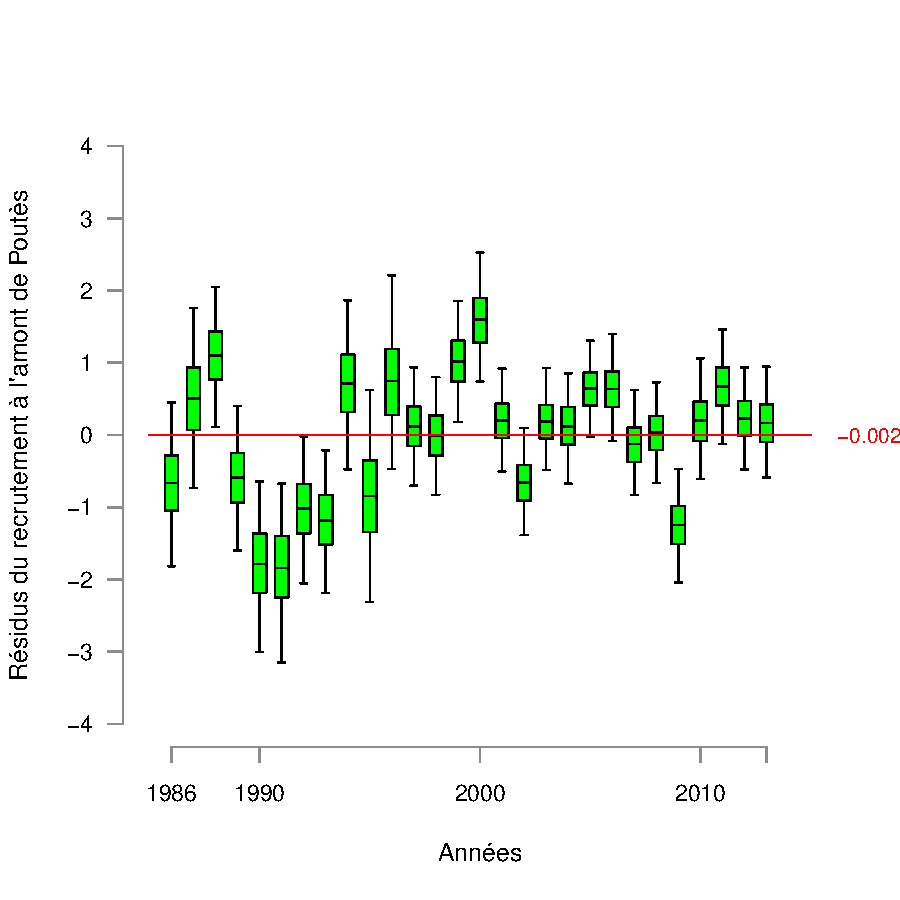
\includegraphics{C:/Users/LOGRAMI/workspace/ModeleDynamiquePop/img/2016_12_19_Alagnon/res_p_poutes.png}%{a_juv.png}
     \caption{res\_p\_poutes}
     \label{res_p_poutes} 
\end{figure}

\clearpage

%=================================================================================
\section{res\_vichy}
%================================================================================

\begin{figure}[ht]
     \includegraphics{C:/Users/LOGRAMI/workspace/ModeleDynamiquePop/img/2016_12_19_Alagnon/res_vichy.png}%{a_juv.png}
     \caption{res\_vichy}
     \label{res_vichy} 
\end{figure}

\clearpage

%=================================================================================
\section{zone\_effect}
%================================================================================
%-------------------------------------------
\subsection{zone\_effect\_Vichy}
%-------------------------------------------

\begin{figure}[ht]
     \includegraphics{C:/Users/LOGRAMI/workspace/ModeleDynamiquePop/img/2016_12_19_Alagnon/zone_effect_V.png}%{a_juv.png}
     \caption{zone\_effect\_V}
     \label{zone_effect_V} 
\end{figure}
\clearpage


\begin{figure}[ht]
     \includegraphics{C:/Users/LOGRAMI/workspace/ModeleDynamiquePop/img/2016_12_19_Alagnon/zone_effect_A.png}%{a_juv.png}
     \caption{zone\_effect\_A}
     \label{zone_effect_A} 
\end{figure}
\clearpage


%-------------------------------------------
\subsection{zone\_effect\_Langeac}
%-------------------------------------------

\begin{figure}[ht]
     \includegraphics{C:/Users/LOGRAMI/workspace/ModeleDynamiquePop/img/2016_12_19_Alagnon/zone_effect_L.png}%{a_juv.png}
     \caption{zone\_effect\_L}
     \label{zone_effect_L} 
\end{figure}
\clearpage
%-------------------------------------------
\subsection{zone\_effect\_Poutes}
%-------------------------------------------

\begin{figure}[ht]
     \includegraphics{C:/Users/LOGRAMI/workspace/ModeleDynamiquePop/img/2016_12_19_Alagnon/zone_effect_P.png}%{a_juv.png}
     \caption{zone\_effect\_P}
     \label{zone_effect_P} 
\end{figure}

\clearpage

%====================================
\section{N\_Vichy}
%====================================

\begin{figure}[ht]
     \includegraphics{C:/Users/LOGRAMI/workspace/ModeleDynamiquePop/img/2016_12_19_Alagnon/N_vichy.png}%{a_juv.png}
     \caption{N\_vichy}
     \label{N_vichy} 
\end{figure}

\clearpage

%====================================
\section{N\_Alagnon}
%====================================

\begin{figure}[ht]
     \includegraphics{C:/Users/LOGRAMI/workspace/ModeleDynamiquePop/img/2016_12_19_Alagnon/N_alagnon.png}%{a_juv.png}
     \caption{N\_alagnon}
     \label{N_alagnon} 
\end{figure}

\clearpage

%====================================
\section{N\_Langeac}
%====================================

\begin{figure}[ht]
     \includegraphics{C:/Users/LOGRAMI/workspace/ModeleDynamiquePop/img/2016_12_19_Alagnon/N_langeac.png}%{a_juv.png}
     \caption{N\_langeac}
     \label{N_langeac} 
\end{figure}

\clearpage

%====================================
\section{d\_wild\_moy}
%====================================
%------------------------------------
\subsection{d\_wild\_moy\_Vichy}
%------------------------------------

\begin{figure}[ht]
     \includegraphics{C:/Users/LOGRAMI/workspace/ModeleDynamiquePop/img/2016_12_19_Alagnon/d_wild_moy_V.png}%{a_juv.png}
     \caption{d\_wild\_moy\_V}
     \label{d_wild_moy_V} 
\end{figure}

\clearpage


%------------------------------------
\subsection{d\_wild\_moy\_Alagnon}
%------------------------------------

\begin{figure}[ht]
     \includegraphics{C:/Users/LOGRAMI/workspace/ModeleDynamiquePop/img/2016_12_19_Alagnon/d_wild_moy_A.png}%{a_juv.png}
     \caption{d\_wild\_moy\_A}
     \label{d_wild_moy_A} 
\end{figure}

\clearpage

%------------------------------------
\subsection{d\_wild\_moy\_Langeac}
%------------------------------------

\begin{figure}[ht]
     \includegraphics{C:/Users/LOGRAMI/workspace/ModeleDynamiquePop/img/2016_12_19_Alagnon/d_wild_moy_L.png}%{a_juv.png}
     \caption{d\_wild\_moy\_L}
     \label{d_wild_moy_L} 
\end{figure}

\clearpage

%------------------------------------
\subsection{d\_wild\_moy\_Poutes}
%------------------------------------

\begin{figure}[ht]
     \includegraphics{C:/Users/LOGRAMI/workspace/ModeleDynamiquePop/img/2016_12_19_Alagnon/d_wild_moy_P.png}%{a_juv.png}
     \caption{d\_wild\_moy\_P}
     \label{d_wild_moy_P} 
\end{figure}

\clearpage

%====================================
\section{d\_juv\_moy}
%====================================
%------------------------------------
\subsection{d\_juv\_moy\_Vichy}
%------------------------------------

\begin{figure}[ht]
     \includegraphics{C:/Users/LOGRAMI/workspace/ModeleDynamiquePop/img/2016_12_19_Alagnon/d_juv_moy_V.png}%{a_juv.png}
     \caption{d\_juv\_moy\_V}
     \label{d_juv_moy_V} 
\end{figure}

\clearpage

%------------------------------------
\subsection{d\_juv\_moy\_Alagnon}
%------------------------------------

\begin{figure}[ht]
     \includegraphics{C:/Users/LOGRAMI/workspace/ModeleDynamiquePop/img/2016_12_19_Alagnon/d_juv_moy_A.png}%{a_juv.png}
     \caption{d\_juv\_moy\_A}
     \label{d_juv_moy_A} 
\end{figure}

\clearpage

%------------------------------------
\subsection{d\_juv\_moy\_Langeac}
%------------------------------------

\begin{figure}[ht]
     \includegraphics{C:/Users/LOGRAMI/workspace/ModeleDynamiquePop/img/2016_12_19_Alagnon/d_juv_moy_L.png}%{a_juv.png}
     \caption{d\_juv\_moy\_L}
     \label{d_juv_moy_L} 
\end{figure}

\clearpage

%------------------------------------
\subsection{d\_juv\_moy\_Poutes}
%------------------------------------

\begin{figure}[ht]
     \includegraphics{C:/Users/LOGRAMI/workspace/ModeleDynamiquePop/img/2016_12_19_Alagnon/d_juv_moy_P.png}%{a_juv.png}
     \caption{d\_juv\_moy\_P}
     \label{d_juv_moy_P} 
\end{figure}

\clearpage

%====================================
\section{d\_egg\_moy}
%====================================
%------------------------------------
\subsection{d\_egg\_moy\_Vichy}
%------------------------------------

\begin{figure}[ht]
     \includegraphics{C:/Users/LOGRAMI/workspace/ModeleDynamiquePop/img/2016_12_19_Alagnon/d_egg_moy_V.png}%{a_juv.png}
     \caption{d\_egg\_moy\_V}
     \label{d_egg_moy_V} 
\end{figure}

\clearpage

%------------------------------------
\subsection{d\_egg\_moy\_Langeac}
%------------------------------------

\begin{figure}[ht]
     \includegraphics{C:/Users/LOGRAMI/workspace/ModeleDynamiquePop/img/2016_12_19_Alagnon/d_egg_moy_L.png}%{a_juv.png}
     \caption{d\_egg\_moy\_L}
     \label{d_egg_moy_L} 
\end{figure}

\clearpage

%====================================
\section{res\_wild\_moy}
%====================================
%------------------------------------
\subsection{res\_wild\_moy\_Vichy}
%------------------------------------

\begin{figure}[ht]
     \includegraphics{C:/Users/LOGRAMI/workspace/ModeleDynamiquePop/img/2016_12_19_Alagnon/res_wild_moy_V.png}%{a_juv.png}
     \caption{res\_wild\_moy\_V}
     \label{res_wild_moy_V} 
\end{figure}

\clearpage

%------------------------------------
\subsection{res\_wild\_moy\_Alagnon}
%------------------------------------

\begin{figure}[ht]
     \includegraphics{C:/Users/LOGRAMI/workspace/ModeleDynamiquePop/img/2016_12_19_Alagnon/res_wild_moy_A.png}%{a_juv.png}
     \caption{res\_wild\_moy\_A}
     \label{res_wild_moy_A} 
\end{figure}

\clearpage

%------------------------------------
\subsection{res\_wild\_moy\_Langeac}
%------------------------------------

\begin{figure}[ht]
     \includegraphics{C:/Users/LOGRAMI/workspace/ModeleDynamiquePop/img/2016_12_19_Alagnon/res_wild_moy_L.png}%{a_juv.png}
     \caption{res\_wild\_moy\_L}
     \label{res_wild_moy_L} 
\end{figure}

\clearpage

%------------------------------------
\subsection{res\_wild\_moy\_Poutes}
%------------------------------------

\begin{figure}[ht]
     \includegraphics{C:/Users/LOGRAMI/workspace/ModeleDynamiquePop/img/2016_12_19_Alagnon/res_wild_moy_P.png}%{a_juv.png}
     \caption{res\_wild\_moy\_P}
     \label{res_wild_moy_P} 
\end{figure}

\clearpage

%====================================
\section{res\_juv\_moy}
%====================================
%------------------------------------
\subsection{res\_juv\_moy\_Vichy}
%------------------------------------

\begin{figure}[ht]
     \includegraphics{C:/Users/LOGRAMI/workspace/ModeleDynamiquePop/img/2016_12_19_Alagnon/res_juv_moy_V.png}%{a_juv.png}
     \caption{res\_juv\_moy\_V}
     \label{res_juv_moy_V} 
\end{figure}

\clearpage

%------------------------------------
\subsection{res\_juv\_moy\_Alagnon}
%------------------------------------

\begin{figure}[ht]
     \includegraphics{C:/Users/LOGRAMI/workspace/ModeleDynamiquePop/img/2016_12_19_Alagnon/res_juv_moy_A.png}%{a_juv.png}
     \caption{res\_juv\_moy\_A}
     \label{res_juv_moy_A} 
\end{figure}

\clearpage


%------------------------------------
\subsection{res\_juv\_moy\_Langeac}
%------------------------------------

\begin{figure}[ht]
     \includegraphics{C:/Users/LOGRAMI/workspace/ModeleDynamiquePop/img/2016_12_19_Alagnon/res_juv_moy_L.png}%{a_juv.png}
     \caption{res\_juv\_moy\_L}
     \label{res_juv_moy_L} 
\end{figure}

\clearpage

%------------------------------------
\subsection{res\_juv\_moy\_Poutes}
%------------------------------------

\begin{figure}[ht]
     \includegraphics{C:/Users/LOGRAMI/workspace/ModeleDynamiquePop/img/2016_12_19_Alagnon/res_juv_moy_P.png}%{a_juv.png}
     \caption{res\_juv\_moy\_P}
     \label{res_juv_moy_P} 
\end{figure}

\clearpage
\end{document}
